\documentclass{ctexart}
\usepackage{geometry}
\usepackage{fancyhdr}
\usepackage{graphicx}
\usepackage{booktabs}
\usepackage{amsmath}
\usepackage{tikz}
\usepackage{array}
\usepackage{zhnumber} % change section number to chinese
\renewcommand\thesection{\zhnum{section}}
\renewcommand \thesubsection {\arabic{subsection}}
\CTEXsetup[format={\Large\bfseries}]{section}

\geometry{
    a4paper,
    left=3.18cm,
    right=3.18cm,
    top=2.54cm,
    bottom=2.54cm
}

\pagestyle{fancy}
\fancyhf{}
\renewcommand{\headrulewidth}{0.7pt} % 设置页眉横线粗细
\fancyhead[L]{\kaishu\large 大学物理实验报告} % 在左侧设置页眉文字
\fancyhead[R]{\kaishu\large 哈尔滨工业大学(深圳) } % 在右侧设置页眉文字
\fancyfoot[R]{\raisebox{1\baselineskip}{\thepage}} % 将页数放在右下角


\setlength\headwidth{\textwidth}

\begin{document}

\noindent
\begin{center}
\textbf{
\begin{tabular}{p{2.4cm}p{2.4cm}p{4cm}p{4cm}}
    班级 \hrulefill & 学号 \hrulefill & 姓名 \hrulefill & 教师签字 \hrulefill \\
\end{tabular}
\begin{tabular}{p{6cm}p{3.6cm}p{3.6cm}}
    实验日期 \hrulefill & 预习成绩 \hrulefill & 总成绩 \hrulefill
\end{tabular}
{\noindent}	 \rule[-10pt]{\textwidth}{0.7pt}
}\end{center}

\begin{center}
    \Large \textbf{实验内容 \underline{夫兰克-赫兹实验}}
\end{center}

\section{实验预习}
\subsection{简要叙述波尔的原子能级理论;}
\subsection{描述夫兰克-赫兹的实验原理。}
\newpage
\section{实验现象及原始数据记录}

有$V_{G1K} = 2.10V $、$ V_{filament} = 2.00V$
分别对拒斥电压为$7.08V$和$7.58V$进行记录,记录的数据显示:
\begin{itemize}
    \item 阴极射线电流的周期性变化:当施加一定电压时,阴极射线电流会随着电压的变化呈现出周期性的变化。这种周期性变化是实验中最主要的现象之一。
    \item 电流峰值的出现:在电流的周期性变化图中,观察到一系列明显的峰值。这些峰值对应着气体原子电子的激发态与基态之间的能量差。当电压增加到足够高时,阴极射线的能量使得电子可以克服气体原子的束缚能而激发到激发态,从而减小了阴极射线电流。
    \item 电流谷值的出现:在峰值之间,会观察到一些电流谷值,这些谷值对应着电子从一个激发态返回到基态时的能量释放。在这些区域,电流增加。
    \item 峰值间隔的恒定性:实验观察到,峰值之间的能量差是大致恒定的。暗示原子的能级结构是量子化的。
\end{itemize}

随后以电流为信号源,利用示波器形成图形,观察电流值变化,结果符合记录数据变化规律。

以下为实验数据:

\begin{table}[h]
    \centering
    \caption{记录数据表格}
    \label{tab:data1}
    \begin{tabular}{ c | c c c c c c c c c c c c}
      \toprule
      $\mathbf{U_{G2K}}$  & 6.5  & 7.0  & 7.5  & 8.0  & 8.5  & 9.0  & 9.5  & 10.0  & 10.5  & 11.0  & 11.5  & 12.0\\
      \hline
      \textbf{7.08} & 0.1  & 0.0  & 0.7  & 3.3  & 6.8  & 10.0  & 12.2  & 14.5  & 16.5  & 18.1  & 19.2  & 20.3 \\
      \textbf{7.58} & 0.1  & 0.1  & 0.0  & 0.6  & 3.9  & 7.9  & 10.9  & 14.0  & 16.4  & 18.3  & 19.7  & 21.0 \\
      \hline
      $\mathbf{U_{G2K}}$  & 12.5  & 13.0  & 13.5  & 14.0  & 14.5  & 15.0  & 15.5  & 16.0  & 16.5  & 17.0  & 17.5  & 18.0\\
      \hline
      \textbf{7.08} & 21.2  & 21.9  & 22.6  & 23.2  & 23.6  & 23.9  & 23.9  & 23.7  & 23.0  & 22.0  & 20.7  & 19.0 \\
      \textbf{7.58} & 22.2  & 23.0  & 23.8  & 24.5  & 25.0  & 25.4  & 25.4  & 25.2  & 24.6  & 23.5  & 22.2  & 20.4 \\
      \hline
      $\mathbf{U_{G2K}}$  & 18.5  & 19.0  & 19.5  & 20.0  & 20.5  & 21.0  & 21.5  & 22.0  & 22.5  & 23.0  & 23.5  & 24.0\\
      \hline
      \textbf{7.08} & 17.0  & 15.4  & 14.4  & 14.5  & 15.6  & 17.0  & 19.2  & 21.7  & 23.7  & 25.9  & 27.8  & 29.0 \\
      \textbf{7.58} & 18.3  & 16.4  & 14.6  & 14.0  & 14.7  & 16.0  & 18.3  & 21.0  & 23.2  & 25.8  & 28.0  & 29.6 \\
      \hline
      $\mathbf{U_{G2K}}$  & 24.5  & 25.0  & 25.5  & 26.0  & 26.5  & 27.0  & 27.5  & 28.0  & 28.5  & 29.0  & 29.5  & 30.0\\
      \hline
      \textbf{7.08} & 30.3  & 31.0  & 31.4  & 31.2  & 30.4  & 29.2  & 26.9  & 23.9  & 21.1  & 17.3  & 13.8  & 11.4 \\
      \textbf{7.58} & 31.0  & 32.1  & 32.5  & 32.5  & 31.8  & 30.5  & 28.3  & 25.4  & 22.4  & 18.5  & 14.7  & 11.3 \\
      \hline
      $\mathbf{U_{G2K}}$  & 30.5  & 31.0  & 31.5  & 32.0  & 32.5  & 33.0  & 33.5  & 34.0  & 34.5  & 35.0  & 35.5  & 36.0\\
      \hline
      \textbf{7.08} & 11.0  & 12.5  & 15.7  & 19.3  & 24.0  & 28.4  & 31.6  & 34.8  & 37.1  & 38.5  & 39.5  & 39.7 \\
      \textbf{7.58} & 9.7  & 10.1  & 12.7  & 16.2  & 21.2  & 26.2  & 30.0  & 33.9  & 36.9  & 38.7  & 40.1  & 40.7 \\
      \hline
      $\mathbf{U_{G2K}}$  & 36.5  & 37.0  & 37.5  & 38.0  & 38.5  & 39.0  & 39.5  & 40.0  & 40.5  & 41.0  & 41.5  & 42.0\\
      \hline
      \textbf{7.08} & 39.4  & 38.3  & 36.4  & 35.0  & 30.7  & 26.4  & 22.3  & 17.4  & 13.1  & 10.9  & 11.4  & 14.5 \\
      \textbf{7.58} & 40.5  & 39.6  & 37.8  & 35.6  & 32.2  & 27.9  & 23.8  & 18.7  & 13.8  & 10.1  & 9.0  & 10.5 \\
      \hline
      $\mathbf{U_{G2K}}$  & 42.5  & 43.0  & 43.5  & 44.0  & 44.5  & 45.0  & 45.5  & 46.0  & 46.5  & 47.0  & 47.5  & 48.0\\
      \hline
      \textbf{7.08} & 19.6  & 24.4  & 30.3  & 35.6  & 39.3  & 42.8  & 45.2  & 46.5  & 47.3  & 47.3  & 46.7  & 45.3 \\
      \textbf{7.58} & 14.8  & 19.6  & 26.0  & 32.2  & 36.7  & 41.2  & 44.5  & 46.4  & 47.7  & 48.1  & 47.7  & 46.5 \\
      \bottomrule
    \end{tabular}
\end{table}

\begin{table}[h]
    \centering
    \begin{tabular}{ c | c c c c c c c c c c c c}
      \toprule
      $\mathbf{U_{G2K}}$  & 48.5  & 49.0  & 49.5  & 50.0  & 50.5  & 51.0  & 51.5  & 52.0  & 52.5  & 53.0  & 53.5  & 54.0\\
      \hline
      \textbf{7.08} & 43.0  & 40.4  & 36.5  & 31.8  & 26.5  & 22.0  & 17.5  & 15.3  & 15.9  & 18.8  & 23.5  & 28.1 \\
      \textbf{7.58} & 44.3  & 41.8  & 38.0  & 33.4  & 28.1  & 23.4  & 18.1  & 14.2  & 13.0  & 14.3  & 18.2  & 22.7 \\
      \hline
      $\mathbf{U_{G2K}}$  & 54.5  & 55.0  & 55.5  & 56.0  & 56.5  & 57.0  & 57.5  & 58.0  & 58.5  & 59.0  & 59.5  & 60.0\\
      \hline
      \textbf{7.08} & 33.9  & 39.2  & 43.2  & 47.2  & 50.3  & 52.1  & 53.6  & 54.2  & 54.0  & 53.0  & 51.2  & 48.6 \\
      \textbf{7.58} & 28.8  & 34.9  & 39.4  & 44.5  & 48.5  & 51.1  & 53.2  & 54.3  & 54.5  & 53.8  & 52.2  & 49.8 \\
      \hline
      $\mathbf{U_{G2K}}$  & 60.5  & 61.0  & 61.5  & 62.0  & 62.5  & 63.0  & 63.5  & 64.0  & 64.5  & 65.0  & 65.5  & 66.0\\
      \hline
      \textbf{7.08} & 45.7  & 41.6  & 36.7  & 32.4  & 27.8  & 24.8  & 24.1  & 25.0  & 27.7  & 30.9  & 35.4  & 40.2 \\
      \textbf{7.58} & 47.0  & 43.0  & 38.2  & 33.8  & 28.5  & 24.1  & 22.0  & 21.6  & 23.2  & 25.9  & 30.3  & 35.4 \\
      \hline
      $\mathbf{U_{G2K}}$  & 66.5  & 67.0  & 67.5  & 68.0  & 68.5  & 69.0  & 69.5  & 70.0  & 70.5  & 71.0  & 71.5  & 72.0\\
      \hline
      \textbf{7.08} & 44.2  & 48.6  & 52.5  & 55.2  & 57.8  & 59.6  & 60.6  & 60.9  & 60.3  & 59.0  & 57.2  & 54.2 \\
      \textbf{7.58} & 39.7  & 44.7  & 49.3  & 52.6  & 55.9  & 58.4  & 59.7  & 60.5  & 60.4  & 59.4  & 57.8  & 55.2 \\
      \hline
      $\mathbf{U_{G2K}}$  & 72.5  & 73.0  & 73.5  & 74.0  & 74.5  & 75.0  & 75.5  & 76.0  & 76.5  & 77.0  & 77.5  & 78.0 \\
      \hline
      \textbf{7.08} & 50.5  & 47.0  & 42.7  & 39.3  & 37.3  & 36.0  & 36.2  & 37.4  & 39.8  & 42.9  & 45.9  & 49.8 \\
      \textbf{7.58} & 51.6  & 48.2  & 43.6  & 39.2  & 36.3  & 34.1  & 33.2  & 33.6  & 35.4  & 38.3  & 41.2  & 45.2 \\
      \hline
      $\mathbf{U_{G2K}}$  & 78.5  & 79.0  & 79.5  & 80.0  & 80.5  & 81.0  & 81.5  & 82.0  & 82.5  & 83.0  & 83.5  & 84.0\\
      \hline
      \textbf{7.08} & 53.6  & 56.8  & 60.2  & 63.1  & 65.5  & 67.0  & 68.2  & 68.6  & 68.3  & 67.2  & 65.3  & 63.1 \\
      \textbf{7.58} & 49.3  & 52.8  & 56.7  & 60.2  & 63.2  & 65.1  & 66.7  & 67.2  & 67.7  & 67.1  & 65.5  & 63.6 \\
      \hline
      $\mathbf{U_{G2K}}$  & 84.5  & 85.0  & 85.5  & 86.0  & 86.5  & 87.0  & 87.5  & 88.0  & 88.5  & 89.0  & 89.5  & 90.0\\
      \hline
      \textbf{7.08} & 60.2  & 57.3  & 55.0  & 52.8  & 51.3  & 50.8  & 50.9  & 52.2  & 53.4  & 55.4  & 56.2  & 56.7 \\
      \textbf{7.58} & 60.7  & 57.4  & 54.7  & 51.9  & 49.6  & 48.5  & 48.0  & 48.4  & 49.4  & 51.1  & 51.8  & 52.3 \\
      \bottomrule
    \end{tabular}
\end{table}

\newpage
\begin{tikzpicture}[remember picture,overlay]
    \node[anchor=south east,inner sep=100pt] at (current page.south east) {
        \renewcommand{\arraystretch}{1.5} % 表格行高倍数
        \setlength{\tabcolsep}{18pt}    
    \begin{tabular}{|c|c|}
        \hline
        \LARGE  教师 & \LARGE  姓名 \\
        \hline
        \LARGE \kaishu 签字 &  \\
        \hline
        \end{tabular}
    };
\end{tikzpicture}

\newpage

\section{数据处理}

\subsection{利用计算机软件绘制$I_A{-{}}U_{G2K}$曲线;}

对实验中记录的数据利用python的matplotlib进行图像绘制,绘制结果如图:

\begin{figure}[h]
    \centering
    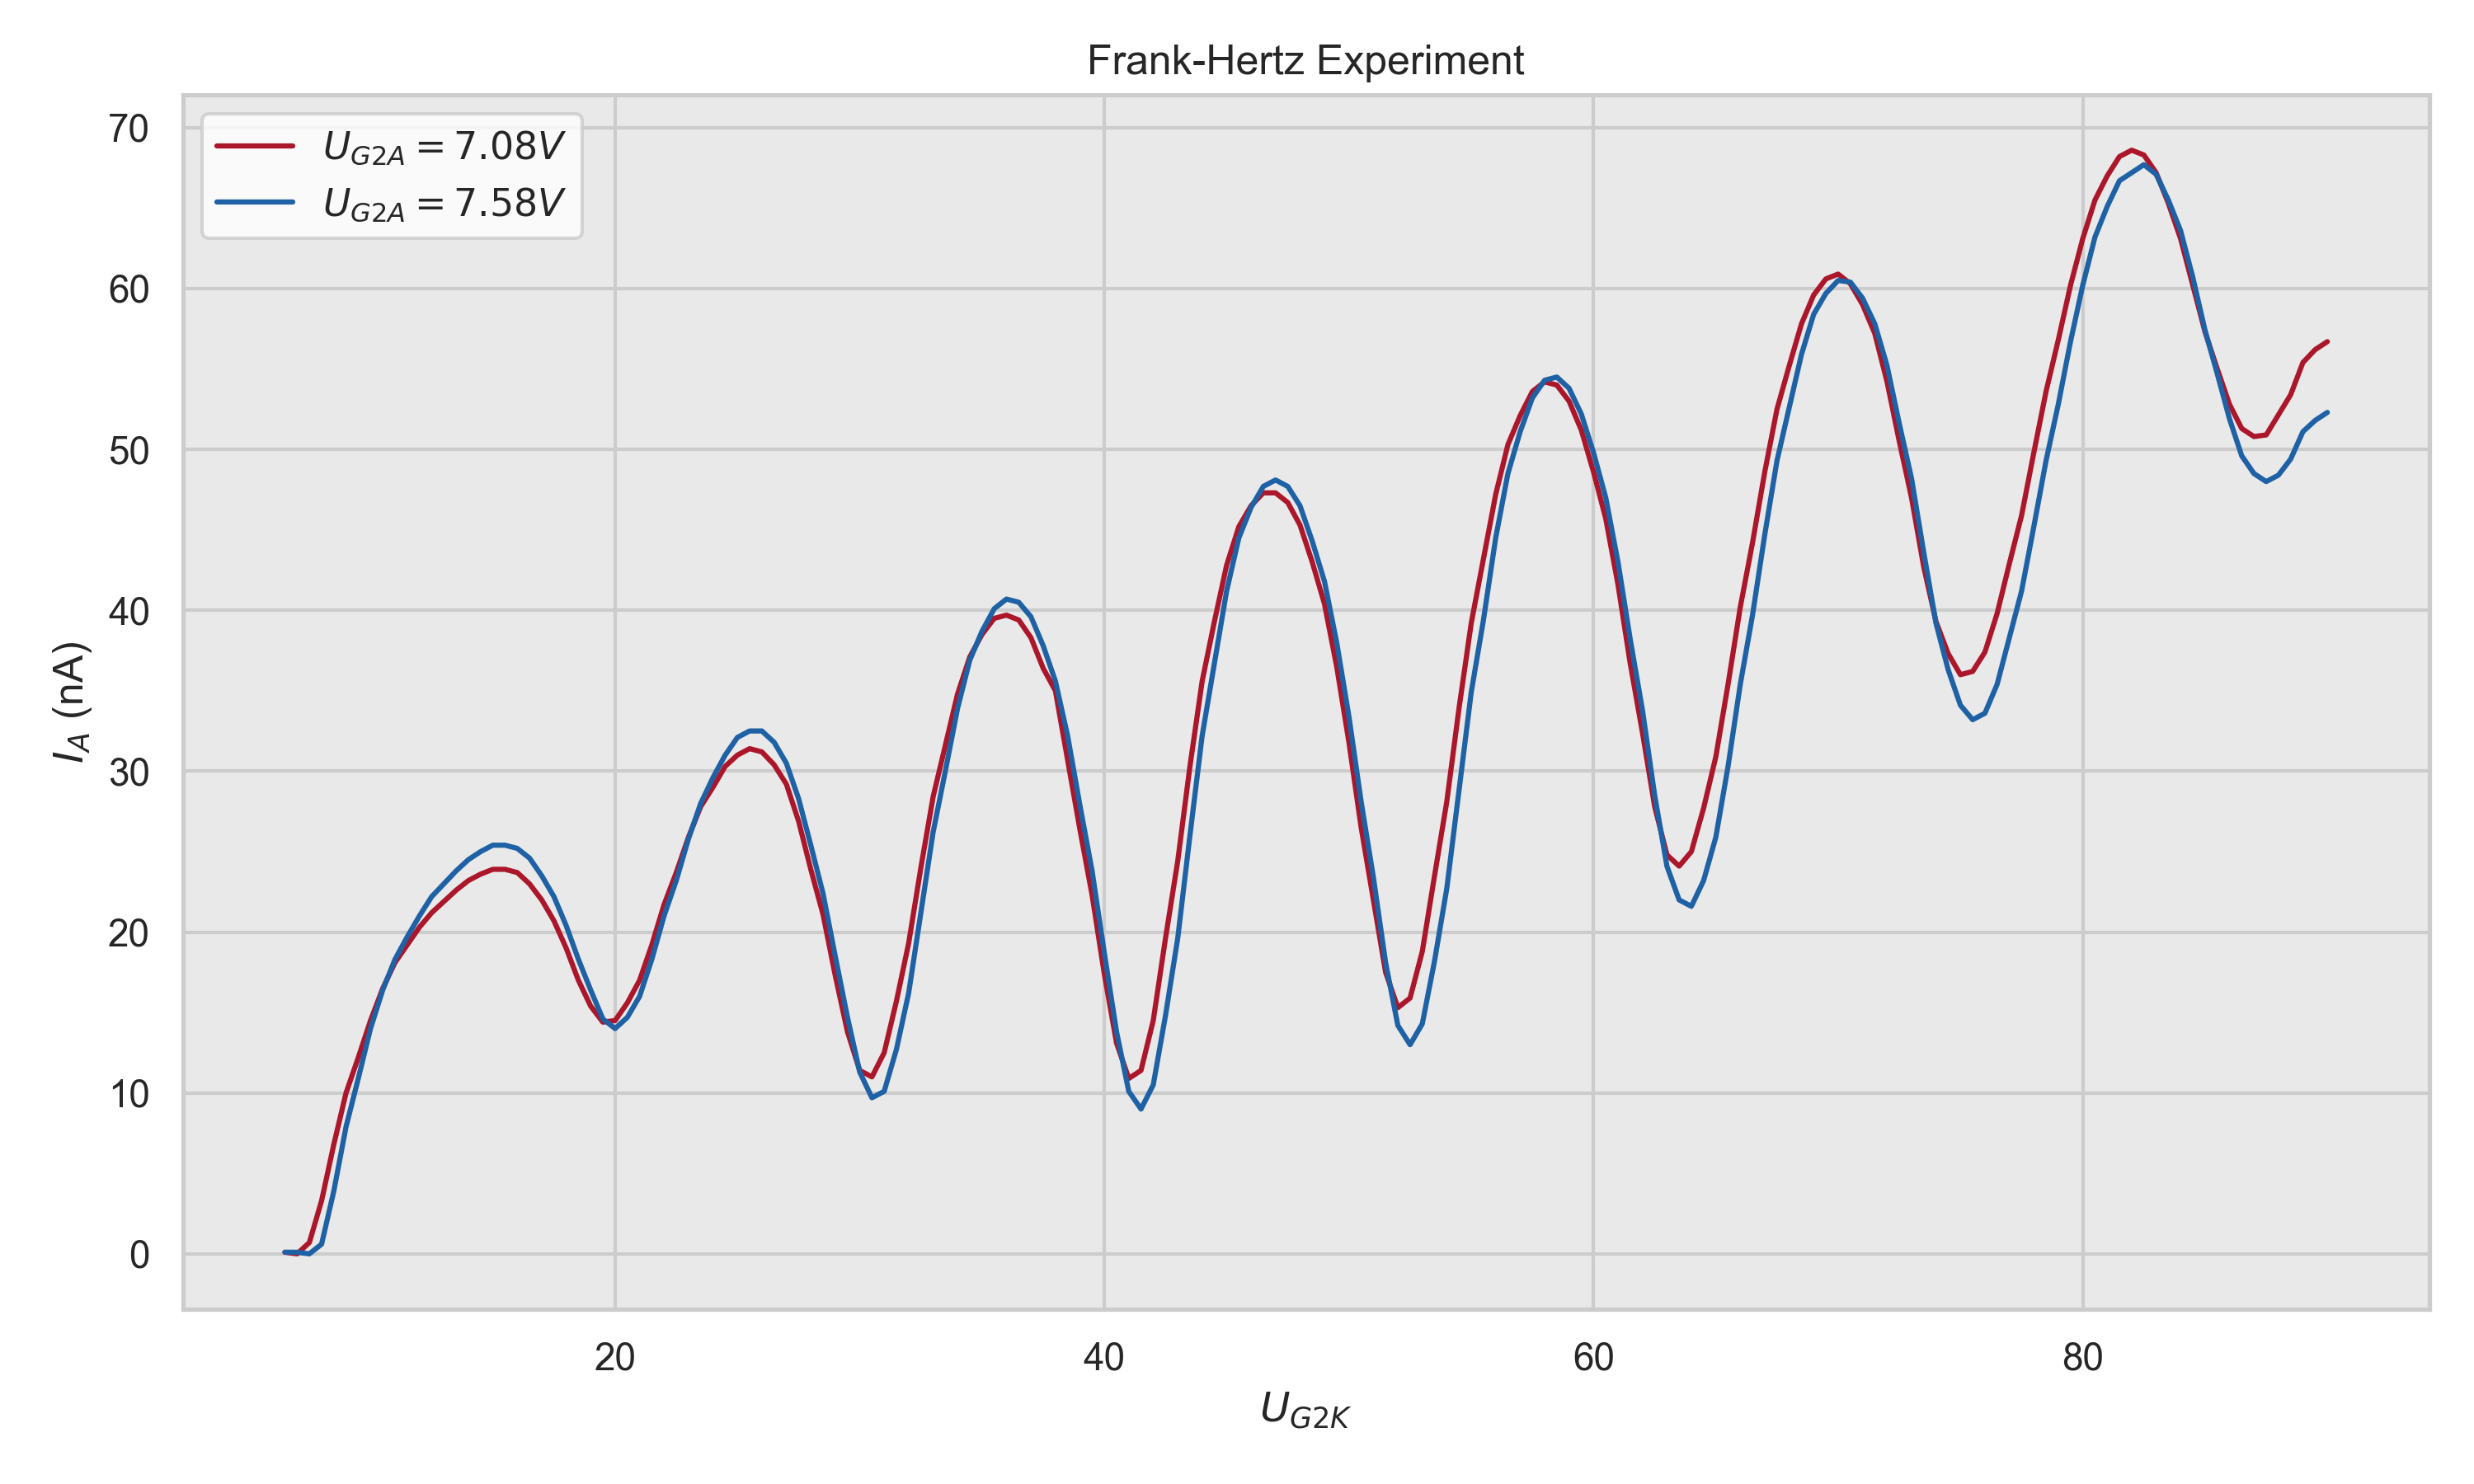
\includegraphics[width=\textwidth]{data.png} % 插入左侧图像
    \caption{绘制的$I_A{-{}}U_{G2K}$曲线}
    \label{fig: data}
\end{figure}

\subsection{对曲线进行拟合,利用各峰值或波谷所对应的电压值,分别用逐差法和最小二乘法计算氩原子的第一激发电位。}

利用scipy的find\_peaks进行寻峰,得到峰值对应$U_{G2K}$值,画得图标并输出统计信息如下所示:

\begin{figure}[h]
    \centering
    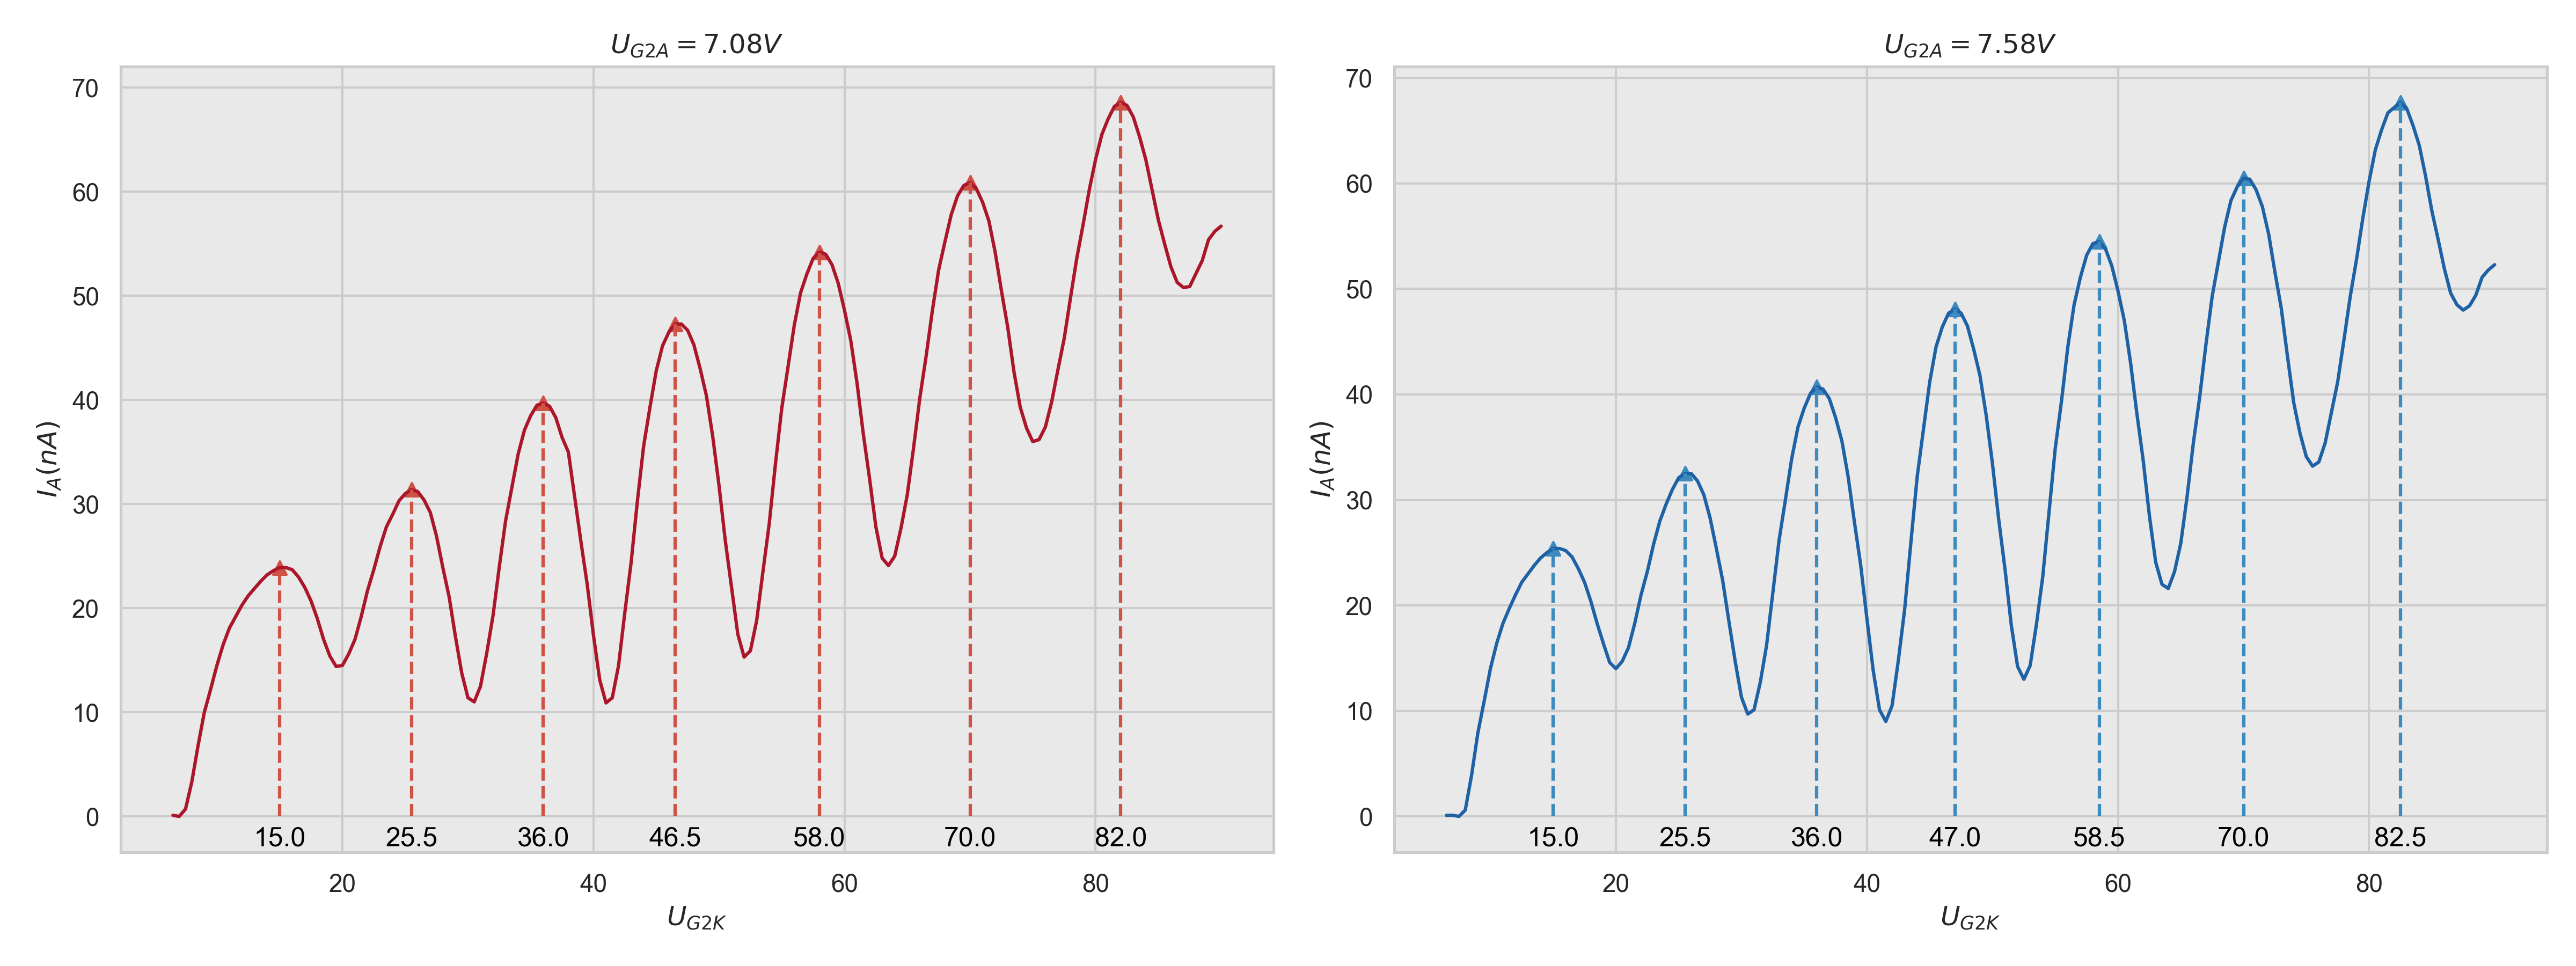
\includegraphics[width=\textwidth]{data-2.png} % 插入左侧图像
    \caption{峰值曲线}
    \label{fig: data-2}
\end{figure}

\begin{table}[h]
    \centering
    \caption{峰值电压值(V)}
    \label{tab:peaks}
    \begin{tabular}{ c | c c c c c c c }
      \toprule
      $\mathbf{U_{G2K}}$  & $U_0$ & $U_1$ & $U_2$ & $U_3$ & $U_4$ & $U_5$ & $U_6$   \\
      \hline
      \textbf{7.08} & 15.0 & 25.5 & 36.0 & 46.5 & 58.0 & 70.0 & 82.0 \\
      \textbf{7.58} & 15.0 & 25.5 & 36.0 & 47.0 & 58.5 & 70.0 & 82.5 \\
      \bottomrule
    \end{tabular}
\end{table}

利用逐差法进行计算,由于得到的数据为奇数个,同时考虑到数据值较小的时候,误差可能会更大,于是舍去小数据进行计算:

$$
\Delta \overline{U} = \frac{1}{3^2} \sum_{i=1}^{3}(U_{i+3}-U_i)
$$

对两组数据进行计算分别得到:

$$
\left\{
\begin{aligned}
    \Delta \overline{U_{7.08}} = 11.33 \\ \
    \Delta \overline{U_{7.58}} = 11.39 
\end{aligned} 
\right.
$$

此时算得其第一电离能为$11.36eV$

利用最小二乘法进行计算,在python中矩阵计算较为方便,所以使用与教材所给公式等价的方式进行计算:


$$ 
A = {\begin{bmatrix}
    1 & 1 & \cdots & 1 \\
    1 & 2 & \cdots & 6 
 \end{bmatrix}}^T \ \ \ \
  Y = {\begin{bmatrix} U_1  & U_2 & \cdots & U_6 \end{bmatrix}}^T
$$

带入公式:
$$ 
\widehat{K} = {(A^T A)}^{-1} A^T Y 
$$

其中$ \widehat{K} = {\begin{bmatrix} k_0  & k_1 & \cdots & k_{n-1} & k_{n} \end{bmatrix}}^T $ 即为所求。

~

计算得:
$$\widehat{K_{7.08}} = \begin{bmatrix} 13.40 \\ 11.31 \end{bmatrix}  \ \ \ \widehat{K_{7.58}} = \begin{bmatrix} 13.40 \\ 11.38 \end{bmatrix}$$

此时算得其第一电离能为$11.34eV$

根据文献数据,氩原子的第一激发电位约为 $11.5 eV$。计算相对误差:

$$
E_R = \frac{|11.34-11.5|}{11.5} \times 100\% = 1.39\%
$$

通过比较

误差在允许范围内,通过逐差法和最小二乘法计算得到的结果 $11.36 eV$ 和 $11.34 eV$ 都与理论值相当接近。这表明我们的实验测量和数据处理是可靠的,并且得到了合理的结果。
\newpage

\section{现象分析及实验结论}

\subsection{现象分析:}
\begin{itemize}
    \item 当施加的电压较小时,加速电子能量过小,不能越过拒斥电场,不会引起明显的能级跃迁。
    \item 随着电压增加,当加速电压高于拒斥电压时,开始出现较明显的电流,并随着加速电压增大而增大。由于被加速的电子只能获得一点点能量,他们只能与氩原子进行纯弹性碰撞。这是因为量子力学不允许一个原子吸收任何能量,除非碰撞能量大于将电子跃迁至较高的能量量子态所需的能量。
    \item 当电压达到一定值时,电子所带的能量足够使得氩原子跃迁到第一激发态,部分电子能量被吸收,导致电流减小,随后电压的增大又使电流继续增大。
    \item 当电子的能量再增加氩原子第一激发能的$n$倍时,发生$n+1$次碰撞,会出现先减后增的现象,形成众多峰。
\end{itemize}

\subsection{结论:}

该实验对\textit{尼尔斯·玻尔}的能级理论提供了强有力的支撑:在\textit{玻尔}创建的玻尔模型里,电子是绕着原子核运行于离散能级的轨道。而实验显示出,原子的确只能够吸收(受激)特定数量的能量(量子),因此证实了玻尔原子的能级是离散的。

\section{讨论题}

\subsection{在$I_A{-}U_{G2K}$曲线中,为什么随着$U_{G2K}$的增大,波谷电流逐渐增大?}

波谷的物理意义即为电子的能量增加了氩原子第一激发能的整数倍,发生了多次碰撞,但是某些电子逃避了碰撞,穿过栅极而到达板极,随着$U_{G2K}$的增大,这些电子的能量增大,因此在$I_A{-}U_{G2K}$曲线上的各谷点电流也随着增大。

\subsection{请分析拒斥电压改变对$I_A-U_{G2K}$曲线的影响。}

由于反向电压增大,所以在任何情况下抵达极板的电子都会减少,故$I_A-U_{G2K}$曲线整体要向下移动。

经过查询资料,了解到加热灯丝溢出电子是热力学平衡的结果,符合麦克斯韦分布(概率密度是能量E的函数),经过加速电场后,分布平移,只有$E \geq e U_{G2A}$ 且没有在碰撞或多次碰撞中使得原子跃迁的电子才能达到极板,在能量密度分布函数中,当$U$的某些值使得$V_{G2K}-U$所夹的面积最大时,$I_A{-}U_{G2K}$曲线出现峰值,由于拒斥电压增大,需要U增大来弥补其变化带来的面积减小,故波峰向右偏移,同理波谷也向右偏移。
\subsection{为什么弗兰克-赫兹实验只能测出第一激发态电位?}
首先原子在激发态是不稳定的,短时间后会回到基态,并以辐射形式释放能量。由于电子加速区与碰撞区重叠,激发更高激发电位需要电子更多能量,而弗兰克赫兹管中填充的氩气很稀薄,无法满足在短时间内电子大量与氩原子碰撞。
\end{document}